%!TEX root = ../rapport.tex
%!TEX encoding = UTF-8 Unicode

% Chapitres "Introduction"

% modifié par Francis Valois, Université Laval
% 31/01/2011 - version 1.0 - Création du document


\label{s:experimentation}
\chapter{Laboratoire 6}
\section{Projet 1: Étalonnage de l'affaiblisseur réglable}
Sachant que nous voulons tracer la courbe de son affaiblissement en fonction de la position de la bande longitudinale, il suffit dans un premier temps d'effectuer une mesure de référence pour régler le ROS-Mètre et par la suite effectuer différentes mesures en modifiant la position de la bande longitudinale. 
Ainsi, à l'aide des méthodes décrites dans le laboratoire \#4, nous avons réglé le ROS-Mètre aux niveaux nécessaires pour obtenir des mesures fonctionnelles, c'est-à-dire une mesure entre -40 et -60 dB, en ajustant la largeur de bande minimale et les différents gains au niveau de la source de tension pour la diode de Gunn et de l'entrée du ROS-Mètre. 

À l'aide du ROS-Mètre maintenant calibré, il est possible d'effectuer les mesures pour différentes position de bande longitudinale entre 0 et 3 mm. Les valeurs obtenues sont affichées dans le tableau \ref{tab:etalonnage_affaib}. Avec ces resultats, il est possible d'obtenir la courbe d'affaiblissement de l'affaiblisseur réglable. Cette courbe est présenté à la figure \ref{fig:affaiblissement}.

En comparant avec les valeurs usuelles fournies dans l'énoncé du laboratoire, nous avons des résultats au dessus des étendues habituelles pour les distances en  
déça de 1mm. Toutefois, nous sommes dans les bonnes intervales au delà de ce point. Ceci peut-être dû à des erreurs de lectures lors des premières prises de mesures mais les différences restent minimes ce qui ne devrais pas impacter les résultats obtenues dans les prochaines sections.
 \begin{table}[htbp]
  \centering
    \begin{tabular}{|c||c|c|} \hline
   Position [mm] & Affaiblissement (Lecture ROS-Mètre) [dB] & Affaiblissement réel [dB]\\ \hline \hline 
Référence & -40,8 & 0\\  
0 & -41,6 & -0,8\\ 
0,25 & -41,9 & -1,1\\ 
0,5 & -42,55 & -1,75\\ 
0,75 & -43,5 & -2,7\\ 
1 & -44,5 & -3,7\\ 
1,25 & -45,75 & -4,95\\ 
1,5 & -47 & -6,2\\ 
1,75 & -48,5 & -7,7\\ 
2 & -50,7 & -9,9\\ 
2,25 & -52,4 & -11,6\\ 
2,5 & -54 & -13,2\\ 
2,75 & -55,5 & -14,7\\ 
3 & -56,7 & -15,9\\ \hline 
    \end{tabular}%
      \caption{Résultats obtenus lors de l'étalonnage de l'affaiblisseur réglable}
  \label{tab:etalonnage_affaib}%
\end{table}%

\begin{figure}[htbp]
    \centering
    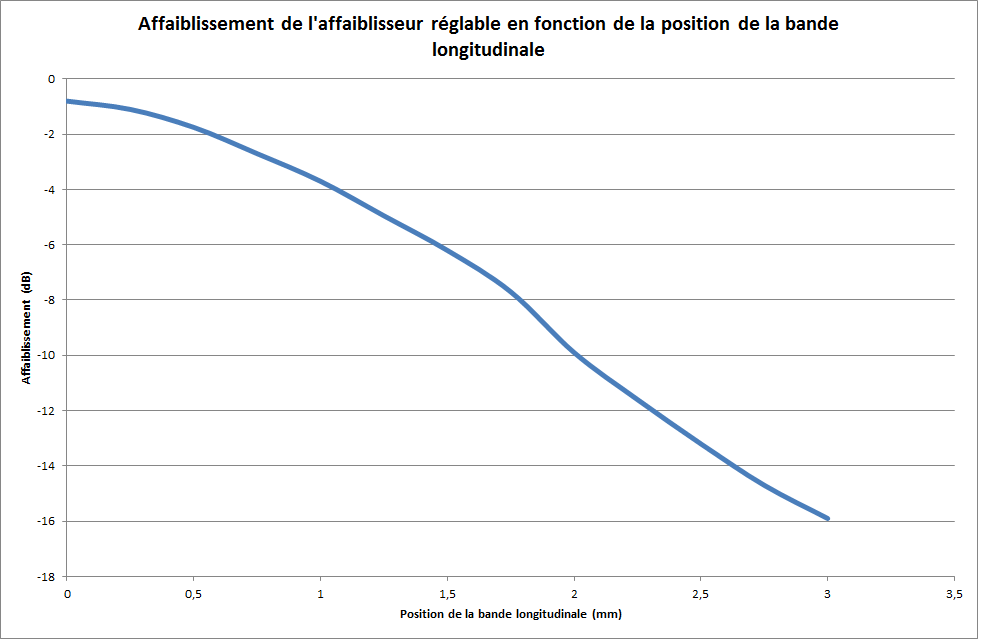
\includegraphics[scale=0.45]{figure1.png}
    \caption{Figure présentant l'affaiblissement de l'affaiblisseur réglable en fonction de la position de la bande longitudinale}
    \label{fig:affaiblissement}
\end{figure}

\section{Projet 2: Mesure du SWR et de la longueur d'onde}
Les résultats obtenus pour l'expérience sur la mesure des différents SWR demandés sont présentés dans les tableaux \ref{tab:tabnum2.1} et \ref{tab:tabnum2.2}.


\subsection{Calcul de la longueur d'onde et de la vitesse de propagation pour un court-circuit}
Il est demandé d'identifier expérimentalement, au moyen du court-circuit la longueur d'onde et la vitesse de propagation du signal dans le guide d'onde. Il est possible d'obtenir la longueur d'onde dans le guide à l'aide de deux méthodes: soit la distance entre deux minimums de l'onde ou la distance entre un maximum et un minimum. Tout dépendant des conditions du systèmes, la précision de chacune des méthodes va varier. Mais en principe, comme les mesures que nous effectuons dépendent de la variation de V(d) autour des points $d_{min}$ et $d_{max}$ et que cette variation est plus importante autour de $d_{min}$, il est plus simple de prendre des mesures précises. C'est pourquoi nous avons utilisé la méthode des minimas.

On sait premièrement que la longueur d'onde est donnée par l'équation suivante:
\begin{equation}
    \lambda_f = 2(d_{min_1} - d_{min_2})
\end{equation}

On sait aussi que la vitesse de propagation dans le guide est donnée par:
\begin{equation}
\label{eq:eq1}
    v_{p_z} = f_o\lambda_f
\end{equation}
Où $f_o$ est la fréquence d'opération de l'onde dans le guide qui est dans notre cas située autour de $10.7 GHz$.

\begin{table}[htbp]
    \centering
    \begin{tabular}{|c||c|c|} \hline
        $d_{min}$ [mm] & Longueur d'onde $\lambda_f$ [m] & Vitesse de propagation [$m/s$]\\ \hline \hline
        36 &  & \\ 
        46 & 0.02 & $2.14\cdot 10^8$\\ 
        56 & 0.02 & $2.14\cdot 10^8$\\ 
        66 & 0.02 & $2.14\cdot 10^8$\\ 
        76 & 0.02 & $2.14\cdot 10^8$\\ 
        87 & 0.022 & $2.354\cdot 10^8$\\ 
        97.5 & 0.021 & $2.247\cdot 10^8$\\ 
        107.8 & 0.0206 & $2.2042\cdot 10^8$\\ \hline
    \end{tabular}%
        \caption{Résultats obtenus lors des différentes prise de mesures de minimas à l'aide d'une charge en court-circuit}
    \label{tab:tabnum2.1}%
\end{table}%
Selon le tableau \ref{tab:tabnum2.1}, on a une longueur d'onde oscillant entre $20cm$ et $22cm$ tout dépendant de quel minimum nous utilisons. Pour obtenir une meilleure précision, utiliser la moyenne de toutes les longueurs d'onde obtenues semble être un choix judicieux et ceci donne une longueur d'onde moyenne de $20.51cm$. Par la suite, en utilisant l'équation \ref{eq:eq1} avec cette valeur, il est possible de trouver une vitesse de propagation moyenne de $2.195 \cdot 10^8 m/s$.

\subsection{Calcul du SWR pour une charge inconnue}
Afin de déterminer le SWR, on applique le développement suivant:
\begin{equation}
\label{eq:3}
SWR = \frac{V_{max}}{V_{min}}
\end{equation}

Pour obtenir, une bonne précision, nous effectuons le calcul du SWR pour les 3 différents cas de minimums et maximums et ensuite nous utilisons la moyenne de ceux-ci pour obtenir le SWR pour cette charge. Dans notre cas, à l'aide des 3 valeurs, nous trouvons un SWR moyen de 1.33.

\begin{table}[htbp]
    \centering
    \begin{tabular}{|c|c||c|c|c|} \hline
       \multicolumn{2}{|c||}{Cas}  & Position [$mm$] & Tension [$dB$] & SWR\\ \hline \hline
\multirow{2}{*}{1} & Maximum & 39 & -53.5 & 0.9\\ 
 & Minimum & 44 & -54.4 & \\ \hline
\multirow{2}{*}{2} & Maximum & 48.2 & -53 & -0.1\\ 
 & Minimum & 54 & -52.9 & \\ \hline
\multirow{2}{*}{3} & Maximum & 60 & -52.9 & 2.6\\ 
 & Minimum & 65.7 & -55.5 & \\ \hline
    \end{tabular}%
        \caption{Résultats obtenus lors des différentes prises de mesures de minimas et maximas à l'aide d'une charge inconnue}
    \label{tab:tabnum2.2}%
\end{table}%

\section{Projet 3: Impédance d'un affaiblisseur court-circuité}
Les données sont présentées au tableau \ref{tab:3} pour la méthode des SWR et au tableau \ref{tab:4} pour la méthode de ligne à pertes.

Pour trouver les deux positions de la bande longitudinale nécessaires pour l'obtention d'une atténuation de 1.5 et 5 dB, nous avons utilisé une extrapolation polynomiale d'ordre 3 de la courbe obtenue à la première section. Cette extrapolation donne respectivement une distance de 0.444 mm et 1.256 mm pour les cas 1.5 et 5 dB. Pour information, l'extrapolation obtenue est représenté par l'équation \ref{eq:2}.

\begin{equation}
\label{eq:2}
    y = 0.5259\cdot x^3 - 3.2643\cdot x^2 + 0.0096\cdot x - 0.9049
\end{equation}
\subsection{Méthode du SWR}

\begin{table}[htbp]
    \centering
    \begin{tabular}{|c|c||c|c|c|c|c|} \hline
    \multicolumn{2}{|c||}{Cas} & Position [$mm$] & Tension [$dB$] & SWR & $\bar{\Gamma}_c$ & Déphasage [$\,^{\circ}$]\\ \hline \hline 
    \multirow{2}{*}{1.5 dB} & Minimum & 59 & -57.2 & \multirow{2}{*}{6.1} & \multirow{2}{*}{0.7183} & \multirow{2}{*}{-74.708}\\ 
 & Maximum & 66.1 & -51.1 & &  & \\ \hline
\multirow{2}{*}{5 dB} & Minimum & 38 & -56 & \multirow{2}{*}{2.75} & \multirow{2}{*}{0.4667} & \multirow{2}{*}{-109.805}\\ 
 & Maximum & 56 & -53.25 & &  & \\ \hline
    \end{tabular}%
        \caption{Résultats obtenus lors des différentes prises de mesures de minimas et maximas pour un court-circuit avec un atténuateur variable}
    \label{tab:3}%
\end{table}%

Pour obtenir $\bar{\Gamma}_c$, il suffit de trouver le SWR à l'aide de l'équation \ref{eq:2} obtenue dans la partie précédente et par la suite utiliser l'équation suivante:
\begin{equation}
    \bar{\Gamma}_c = \frac{SWR - 1}{SWR + 1}
\end{equation}

 Pour obtenir le déphasage de $\bar{\Gamma}_c$, deux méthodes sont possibles. La première méthode consiste de choisir un minimum obtenue à la section précédente, de placer la ligne fendue à cette position et s'éloigner de la charge jusqu'à retrouver un nouveau minimum. Par la suite, en utilisant l'équation suivante, il est possible de déduire le $d_{min}$ réel:

\begin{equation}
    d_{min_{reel}} = d_{min_{mes}} - d_{min_{\#2}} 
\end{equation}

La deuxième méthode est tout simplement l'inverse de la précédente. Lorsque que la ligne fendue est positionnée sur un minimum obtenu dans la section précédente, il suffit de se rapprocher de la charge jusqu'à trouver un nouveau minimum et utiliser l'équation suivante pour obtenir le $d_{min}$ réel:

\begin{equation}
    d_{min_{reel}} = \frac{\lambda_f}{2} - (d_{min_{\#2}} - d_{min_{mes}}) 
\end{equation}

Pour les deux cas demandés, nous avons choisis la première méthode qui simplifie les calculs et permet d'éviter les erreurs qui pourraient se glisser lors du calcul à l'aide de la longueur d'onde. Ainsi, dans le cas 1.5 dB, nous avons choisi comme $d_{min_{\#2}}$, une position initiale de $56mm$ et dans le second cas, une position initiale de $36mm$. À l'aide de ces valeurs et de celle obtenue lors de la manipulation, nous trouvons les $d_{min_{reel}}$ suivants: 3mm et 2mm.

Par la suite, lorsque la distance réelle entre deux minimas est connue, il suffit d'utiliser l'équation suivante pour obtenir le déphasage en degré:
\begin{equation}
    \xi_c = \frac{720d_{min}}{\lambda_f}-180
\end{equation}

À l'aide de la longueur d'onde moyenne calculée plus tôt, soit $20.51cm$, il est possible de trouver les déphasages suivants: -74.708$\,^{\circ}$ et -109.805$\,^{\circ}$

Finalement, pour trouver l'impédance de charge vu a l'entrée de l'atténuateur, il suffit d'utiliser l'équation suivante:
\begin{equation}
\label{eq:eq6}
    \bar{Z}_c = \frac{1+\bar{\Gamma}_c e^{\xi_c}}{1-\bar{\Gamma}_c e^{\xi_c}}
\end{equation}
Ainsi, en utilisant les valeurs précédemment trouvées, on obtient une impédence de charge de $1.2909 \angle -70.75\,^{\circ}$ pour l'atténuation de 1.5 dB et l'impédance $0.7666 \angle -48.31\,^{\circ}$ pour l'atténuation de 5 dB.

\subsection{Méthode de la ligne à pertes}
Le coefficient de réflexion dans le cas de la ligne à perte est donnée par l'équation suivante :

\begin{equation}
\label{eq:eq5}
     \bar{\Gamma}_c(l) =  (\bar{\Gamma}_c e^{-2Att_{np}}) \angle (\xi_c - 720l_e)
\end{equation}
Où :
\begin{itemize}
    \item $\bar{\Gamma}_c$ est le coefficient de réflexion du court-circuit, dans notre cas -1;
    \item $Att_{np}$ est l'atténuation de la ligne en népers;
    \item $l_e$ est la longueur électrique de la ligne;
    \item $\xi_c$ est le déphasage causé par la charge, dans notre cas $180\,^{\circ}$.
\end{itemize}

Pour obtenir l'atténuation en népers à partir de l'atténuation en décibel, il suffit d'utiliser la règle de trois suivante:
\begin{equation}
    Att_{np} = \frac{Att_{db}}{8.686}
\end{equation}
Pour une atténuation de 1.5 et 5 dB, nous avons respectivement en népers : 0.173 et 0.576.

De plus, pour obtenir la longueur électrique $l_e$, il suffit d'utiliser l'équation suivante:
\begin{equation}
    l_e = \frac{l}{\lambda_f}
\end{equation}
Ainsi, pour une longueur physique de 0.150 m et une longueur d'onde de 0.0205m, nous obtenons une longueur électrique de $7.317\lambda$

En remplaçant dans l'équation \ref{eq:eq5}, nous trouvons les deux coefficients suivants pour les deux différents cas:

\begin{equation}
    \bar{\Gamma}_c(l)_{1.5dB} = e^{-2\cdot 0.173} \angle (180 - 720\cdot 7.317) = 0.70751 \angle -48.24
\end{equation}

\begin{equation}
    \bar{\Gamma}_c(l)_{5dB} = e^{-2\cdot 0.576} \angle (180 - 720\cdot 7.317) = 0.316 \angle -48.24
\end{equation}

En utilisant l'équation suivante, qui est la même que tout à l'heure mais avec des paramètres modifiés, il est possible de trouver les impédences recherchées:

\begin{equation}
    \bar{Z}_c = \frac{1+\bar{\Gamma}_c e^{\angle \bar{\Gamma}_c}}{1-\bar{\Gamma}_c e^{\angle \bar{\Gamma}_c}}
\end{equation}
Ainsi, en utilisant les valeurs précédemment trouvées, on obtient une impédence de charge de $2.0921 \angle -64.68\,^{\circ}$ pour l'atténuation de 1.5 dB et l'impédance $1.4966 \angle -27.64\,^{\circ}$ pour l'atténuation de 5 dB.

\subsection{Comparaison des deux méthodes}
Le tableau \ref{tab:4} reporte les différentes impédances obtenues dans cette section. Comme nous pouvons le remarquer, les deux méthode possèdent un grand écart entre leurs valeurs à la même atténuation. Dans un premier temps, pour expliquer cette différence, il faut expliquer la différence fondamentale entre les deux méthodes. La première méthode est basée sur un test physique qui permet de mesurer le SWR et la longueur d'onde directment au point voulu en tenant compte de tout les paramètres ignorés dans la théorie. La deuxième méthode quand-à elle se base sur plusieurs données théoriques comme l'angle de réflexion et le coefficients du court-circuit parfait et néglige complètement la modification de la vitesse phase du système par l'atténuateur (plus l'atténuation augmente, plus la vitesse de phase devient complexe et apporte de plus en plus d'erreur)et les autres imperfection du guide d'onde utilisé. C'est pourquoi il est tout simplement impossible d'obtenir les même résultats avec les deux méthodes. La première méthode est intéressante si un bon degré de précision est nécessaire et si le montage peut-être testé. La seconde méthode peut-être utilisé pour accélérer les calculs car nous avons besoin seulement de la longueur physique et des fréquences d'utilisations pour obtenir un résultat.

  \begin{table}[htbp]
    \centering
    \begin{tabular}{|c||c|c|} \hline
    Atténuation & Méthode du SWR & Méthode par ligne à pertes \\ \hline  \hline
    1.5 dB & $1.2909 \angle -70.75\,^{\circ}$ & $2.0921 \angle -64.68\,^{\circ}$ \\
    5 dB   & $0.7666 \angle -48.31\,^{\circ}$ & $1.4966 \angle -27.64\,^{\circ}$ \\ \hline
    \end{tabular}%
        \caption{Impédances de charges selon les deux méthodes pour deux différents cas}
    \label{tab:4}%
\end{table}%

\section{Projet 4: Impédance d'un affaiblisseur court-circuité}